\documentclass[12pt]{report}
\usepackage[utf8]{inputenc}
\usepackage[russian]{babel}
%\usepackage[14pt]{extsizes}
\usepackage{listings}
\usepackage{graphicx}
\usepackage{amsmath,amsfonts,amssymb,amsthm,mathtools} 
\usepackage{pgfplots}
\usepackage{filecontents}
\usepackage{float}
\usepackage{comment}
\usepackage{indentfirst}
\usepackage{eucal}
\usepackage{enumitem}
%s\documentclass[openany]{book}
\frenchspacing

\usepackage{array}

\usepackage{verbatim}

\usepackage{caption}
\captionsetup{labelsep=endash}
\captionsetup[figure]{name={Рисунок}}

\usepackage{indentfirst} % Красная строка

\usetikzlibrary{datavisualization}
\usetikzlibrary{datavisualization.formats.functions}

\usepackage{amsmath}


% Для листинга кода:
\lstset{ %
	language=c,                 % выбор языка для подсветки (здесь это С)
	basicstyle=\small\sffamily, % размер и начертание шрифта для подсветки кода
	numbers=left,               % где поставить нумерацию строк (слева\справа)
	numberstyle=\tiny,           % размер шрифта для номеров строк
	stepnumber=1,                   % размер шага между двумя номерами строк
	numbersep=5pt,                % как далеко отстоят номера строк от подсвечиваемого кода
	showspaces=false,            % показывать или нет пробелы специальными отступами
	showstringspaces=false,      % показывать или нет пробелы в строках
	showtabs=false,             % показывать или нет табуляцию в строках
	frame=single,              % рисовать рамку вокруг кода
	tabsize=2,                 % размер табуляции по умолчанию равен 2 пробелам
	captionpos=t,              % позиция заголовка вверху [t] или внизу [b] 
	breaklines=true,           % автоматически переносить строки (да\нет)
	breakatwhitespace=false, % переносить строки только если есть пробел
	escapeinside={\#*}{*)}   % если нужно добавить комментарии в коде
}


\usepackage[left=2cm,right=2cm, top=2cm,bottom=2cm,bindingoffset=0cm]{geometry}
% Для измененных титулов глав:
\usepackage{titlesec, blindtext, color} % подключаем нужные пакеты
\definecolor{gray75}{gray}{0.75} % определяем цвет
\newcommand{\hsp}{\hspace{20pt}} % длина линии в 20pt
% titleformat определяет стиль
\titleformat{\chapter}[hang]{\Huge\bfseries}{\thechapter\hsp\textcolor{gray75}{|}\hsp}{0pt}{\Huge\bfseries}


% plot
\usepackage{pgfplots}
\usepackage{filecontents}
\usetikzlibrary{datavisualization}
\usetikzlibrary{datavisualization.formats.functions}

\begin{document}
	%\def\chaptername{} % убирает "Глава"
	\thispagestyle{empty}
	\begin{titlepage}
		\noindent \begin{minipage}{0.15\textwidth}
			
\includegraphics[width=\linewidth]{inc/b_logo}
		\end{minipage}
		\noindent\begin{minipage}{0.9\textwidth}\centering
			\textbf{Министерство науки и высшего образования Российской Федерации}\\
			\textbf{Федеральное государственное бюджетное образовательное учреждение высшего образования}\\
			\textbf{~~~«Московский государственный технический университет имени Н.Э.~Баумана}\\
			\textbf{(национальный исследовательский университет)»}\\
			\textbf{(МГТУ им. Н.Э.~Баумана)}
		\end{minipage}
		
		\noindent\rule{18cm}{3pt}
		\newline\newline
		\noindent ФАКУЛЬТЕТ $\underline{\text{«Информатика и системы управления»}}$ \newline\newline
		\noindent КАФЕДРА $\underline{\text{«Программное обеспечение ЭВМ и информационные технологии»}}$\newline\newline\newline\newline\newline
		
		\begin{center}
			\noindent\begin{minipage}{1.1\textwidth}\centering
				\Large\textbf{Отчет по лабораторной работе №2}\newline
				\textbf{по дисциплине <<Моделирование>>}\newline\newline
			\end{minipage}
		\end{center}
		
		\noindent\textbf{Тема} $\underline{\text{Марковские цепи}}$\newline\newline
		\noindent\textbf{Студент} $\underline{\text{Слепокурова М.Ф.}}$\newline\newline
		\noindent\textbf{Группа} $\underline{\text{ИУ7-76Б}}$\newline\newline
		\noindent\textbf{Оценка (баллы)} $\underline{\text{~~~~~~~~~~~~~~~~~}}$\newline\newline
		\noindent\textbf{Преподаватель} $\underline{\text{Рудаков И.В.}}$\newline\newline\newline
		
		\begin{center}
			\vfill
			Москва~---~\the\year
			~г.
		\end{center}
	\end{titlepage}

\setcounter{page} {2}





\section*{Постановка задачи}
Определить вероятность и время пребывания системы в каждом состоянии в установившемся режиме работы СМО. Исходные данные: кол-во состояний системы (max 10) и матрица интенсивностей переходов из состояния в состояние.

\section*{Теория}
Случайный процесс, протекающий в сложной системе $S$, называется марковским, если он обладает следующим свойством:  для каждого момента времени $t_0$ вероятность любого состояния системы в будущем при $t > t_0$ зависит только от состояния системы в настоящем $t = t_0$ и не зависит от того, когда и каким образом система перешла в это состояние (как процесс развивался в прошлом). В марковском случайном процессе будущее развитие зависит только от настоящего состояния и не зависит от предыстории процесса.
\newline


Для марковского процесса составлены уравнения Колмогорова:
$$F=(P'(t), P(t), \lambda)=0$$


Вероятностью $i$-го состояния называется вероятность $p_i(t)$ того, что в момент времени $t$ система будет находиться в состоянии $S_i$. Для любого момента $t$ сумма вероятностей всех состояний равна единице. 

Для нахождения предельных вероятностей используется система уравнений вида:

\begin{equation*}
 \begin{cases}
   p'_0 = \lambda_{10}p_1 + \lambda_{20}p_2 - (\lambda_{01} + \lambda_{02})p_0,
   \\
  p'_1 = \lambda_{01}p_0 + \lambda_{31}p_3 - (\lambda_{10} + \lambda_{13})p_1,
   \\
  p'_2 = \lambda_{02}p_0 + \lambda_{32}p_3 - (\lambda_{20} + \lambda_{23})p_2,
  \\
  p'_3 = \lambda_{13}p_1 + \lambda_{23}p_2 - (\lambda_{31} + \lambda_{32})p_3.
 \end{cases}
\end{equation*}
\newline


В левой части каждого из уравнений стоит производная вероятности $i$-го состояния; в правой части - сумма произведений вероятностей всех состояний (из которых идут стрелки в данное состояние), умноженная на интенсивности соответствующих потоков событий, минус суммарная интенсивность всех потоков, выводящих систему из данного состояния, умноженная на вероятность данного $i$-го состояния.
\newline


Так как предельные вероятности постоянны, то, заменяя в уравнениях Колмогорова их производные нулевыми значениями, получим систему линейных алгебраических уравнений, описывающих стационарный режим при $t \rightarrow \infty$.
Для решения полученной системы необходимо добавить условие нормировки $(p_0 + p_1 + p_2 + p_3)$ вместо одного из уравнений.
\newline


После нахождения вероятностей, необходимо вычислить время пребывания системы в каждом из состояний. Для этого необходимо с заданным интервалом $\delta t$ вычислять приращение вероятности для $i$-го состояния по формуле вида:
\begin{equation*}
   dp_0 = (\lambda_{10}p_1 + \lambda_{20}p_2 - (\lambda_{01} + \lambda_{02})p_0) * \delta t,
\end{equation*}

Вычисления завершаются, когда найденная вероятность будет равна соответствующей предельной с точностью до заданной погрешности.
\newline


Для приращения вероятности $dp$ необходимо задать начальные значения, например, $1/n$, где $n$ - число состояний системы.

\section*{Средства реализации}

Для реализации приложения был выбран язык программирования Python, в стандартную библиотеку которого входит графическая библиотека Tkinter, использовавшаяся для реализации пользовательского интерфейса, а также библиотека Numpy, использовавшаяся для решения системы уравнений методом Крамера.

\section*{Листинг кода}

\begin{lstlisting}
from numpy import linalg

TIME_DELTA = 1e-3
EPS = 1e-5

def __getCoefMatrix(matrix):
  count = len(matrix)
  coefMatrix = [[0.0 for j in range(count)] for i in range(count)]

  for i in range(count):
    for j in range(count):
      if (i == j): coefMatrix[i][i] = -sum(matrix[i]) + matrix[i][i] 
      else: coefMatrix[i][j] = matrix[j][i]
  return coefMatrix

def calculateProbability(matrix):
  count = len(matrix)
  coefMatrix = __getCoefMatrix(matrix)
  coefMatrix[count - 1] = [1 for j in range(count)]

  ordinateValues = [0 if i != count - 1 else 1 for i in range(count)]
  return linalg.solve(coefMatrix, ordinateValues).tolist()

def __calculateProbDelta(matrix, probCurr):
  count = len(matrix)
  probDelta = []
  coefMatrix = __getCoefMatrix(matrix)
  for i in range(count):
    for j in range(count):
      coefMatrix[i][j] *= probCurr[j]
    probDelta.append(sum(coefMatrix[i]) * TIME_DELTA)
  return probDelta
\end{lstlisting}
\clearpage
\begin{lstlisting}
def calculateTime(matrix, prob):
  count = len(matrix)
  timeCurr = 0.0
  probCurr = [1.0 / count for i in range(count)]
  time = [0.0 for i in range(count)]
  
  while not all(time):
    probDelta = __calculateProbDelta(matrix, probCurr)
    for i in range(count):
      if not time[i] and abs(probCurr[i] - prob[i]) <= EPS:
        time[i] = timeCurr
      probCurr[i] += probDelta[i]
    timeCurr += TIME_DELTA
  return time
\end{lstlisting}
\section*{Демонстрация работы программы}
На рисунке \ref{fig:pic1} изображен пример работы программы для системы с 5 состояниями.

\begin{figure}[h!btp]
	\centering
	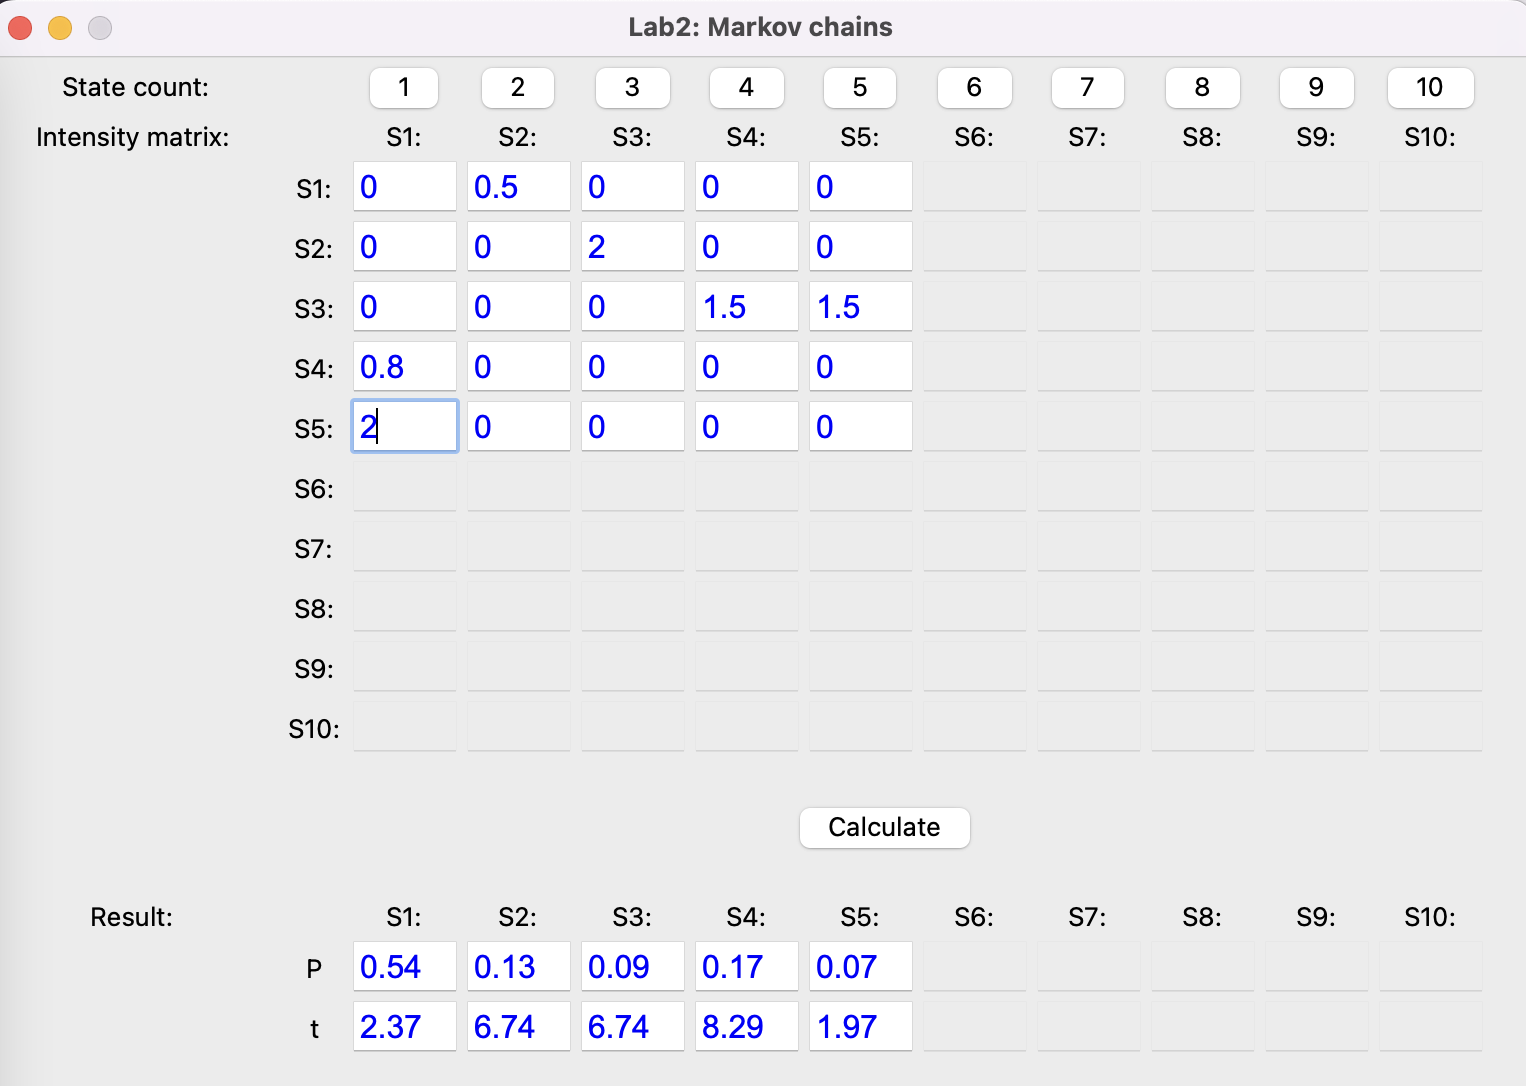
\includegraphics[width=1\textwidth]{inc/pic1.png}
	\caption{Пример работы программы --- 1}
	\label{fig:pic1}	
\end{figure}

\clearpage
На рисунке \ref{fig:pic1} изображен пример работы программы для системы с 2 состояниями.

\begin{figure}[h!btp]
	\centering
	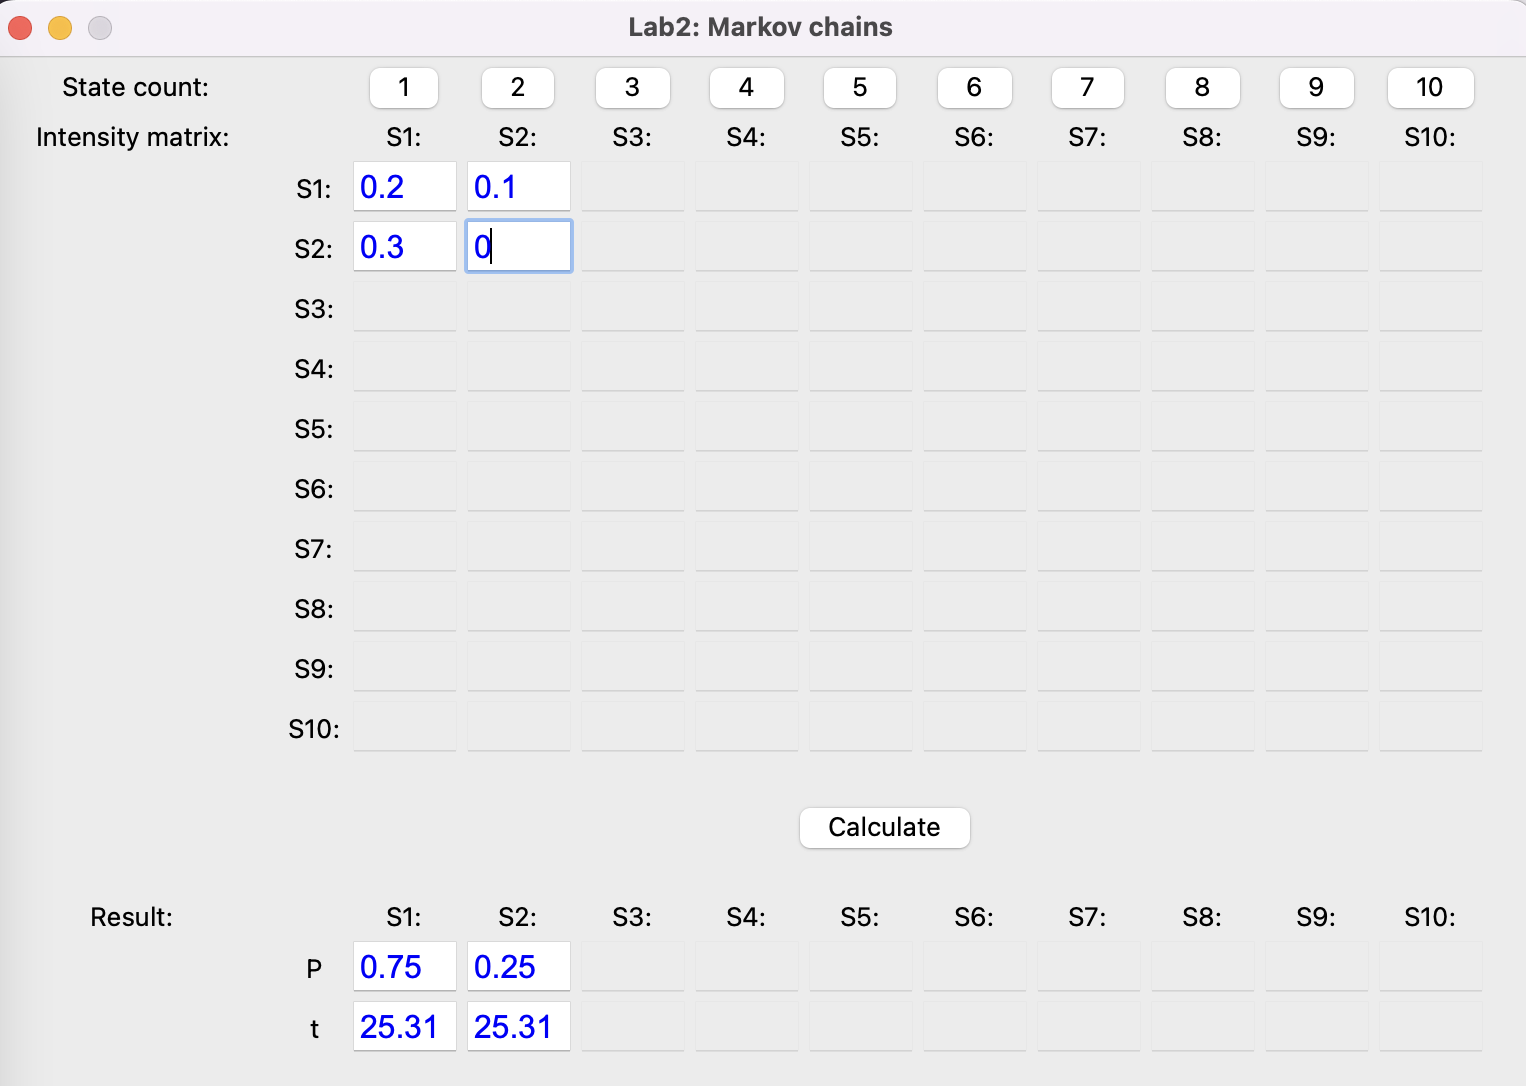
\includegraphics[width=1\textwidth]{inc/pic2.png}
	\caption{Пример работы программы --- 2}
	\label{fig:pic2}	
\end{figure}
\clearpage

На рисунке \ref{fig:pic1} изображен пример работы программы для системы с 10 состояниями.

\begin{figure}[h!btp]
	\centering
	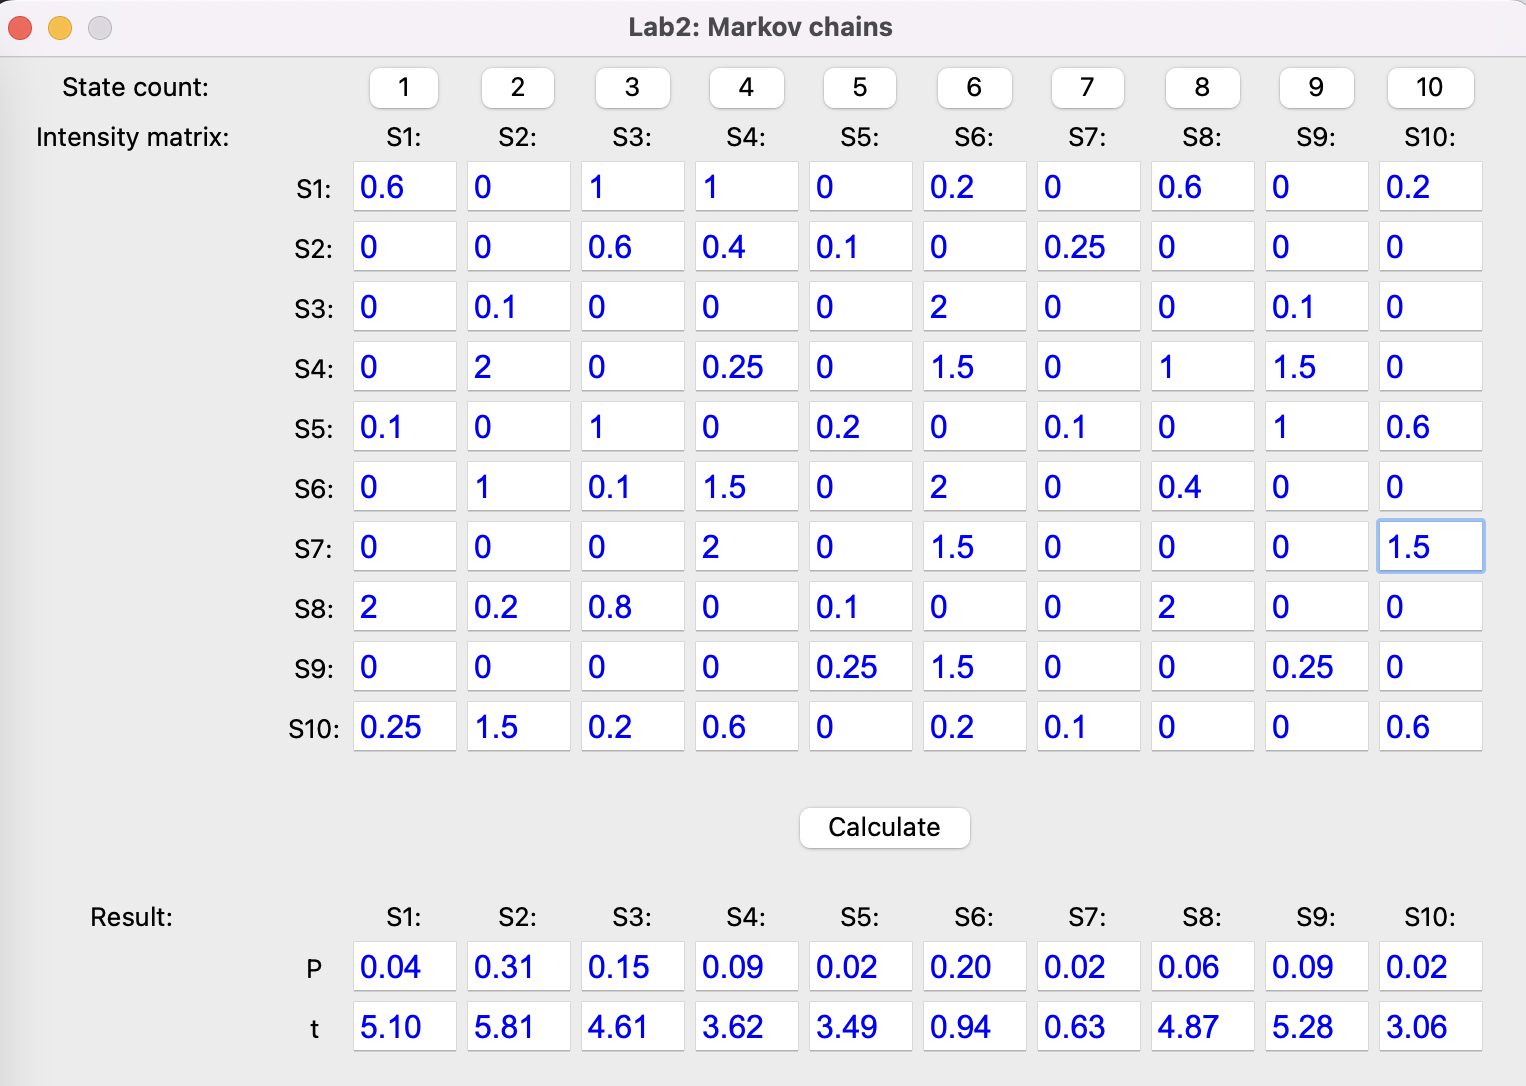
\includegraphics[width=1\textwidth]{inc/pic3.png}
	\caption{Пример работы программы --- 3}
	\label{fig:pic3}	
\end{figure}

\bibliographystyle{utf8gost705u}  % стилевой файл для оформления по ГОСТу
\bibliography{51-biblio}          % имя библиографической базы (bib-файла)
	
\end{document}
